\documentclass[11pt]{article}
\usepackage{fullpage}
\usepackage{graphicx}
\usepackage{subfig}

\title{Multicast Routing Algorithms: Reverse Path Forwarding and Center-Based Trees}
\author{Phyo Thiha and Liang Xin}
\date{April 23, 2013}

\begin{document}
  \maketitle
  \begin{abstract}
    Multicast has become a staple of our browsing experience. Our extensive use of streaming media has motivated large amounts of work into finding the most efficient way to send a single packet to many receivers with as little redundancy as possible. In this project, we explored two of the more well-known approaches: reverse path forwarding and center-based trees. Specifically, we wanted to find out how each used - or abused - network resources, and how quickly each delivered multicast packets. we tested the two algorithms in a variety of small network topologies (twelve nodes or less), recording how many bytes each node sent and received, as well as the average message transmission cost from one source to the other. As predicted, center-based trees make far better use of network resources while suffering a minor penalty in average transmission cost as compared to reverse path forwarding. 
  \end{abstract}
  \newpage
  
  \section{Compilation and Use}
    \subsection{Compiling}
      To compile, run \emph{javac mcast/*.java}.
      
    \subsection{Running}
      To use reverse path forwarding, run \emph{java mcast/RPFNode port file [stats]} on each node, where \emph{stats} is an optional flag for printing the statistical information. To use center-based trees, run \emph{java mcast/CBTNode port file [stats]}. Topology files for testing can be found in the top folder and its subdirectories.
  
  \section{Overview}
    This project originated as project suggestion \#3, which was to implement the reverse path forwarding routing algorithm with pruning as a multicast solution. The program was to include functionality for nodes to join any number of multicast groups, receive messages from these groups, and send out messages to all other group members. We also added commands for removing one's self from a multicast group, as well as sending a random series of bytes to a multicast group (this came in handy for data collection).
    
    Some background research into reverse path forwarding, however, revealed that it was a somewhat cludgy solution for multicast that did not scale well. While it is guaranteed to always use the shortest path to a destination, providing paths from a source to a destination are symmetric, it makes only modest improvements in reducing packet redundancy: that is, it still transmits an unnecessary number of packets, though fewer than the naive flooding implementation of multicast. We make some more modest gains by adding a pruning mechanism, but even so, the general concensus seemed to be that reverse path forwarding only really shined in extremely dense multicast networks.
    
    Center-based tree routing, on the other hand, is a possibly more scalable alternative to reverse path forwarding. While a center-based tree makes no guarantee of using the shortest path route between two group endpoints, the restriction of communication to one group of paths (rather than n-many sets for n nodes) can greatly reduce redundant transmissions.
    
    So, in essence, the choice between reverse path forwarding and center-based tree routing is a choice between low transmission cost and increased throughput, respectively. Because of this discrepancy, we wanted to use this project to not only implement these two algorithms, but to also conduct some light analyses into their total byte expenditures, amount of overhead, and transmission costs. Based on past literature and our intuition, we anticipated that RPF would use far more bytes to send the same amount of actual data as CBT, while CBT's transmission costs would be somewhat higher than RPF's. Would these predictions be supported or refuted, and to what degree? This will be discussed more in the analysis section.
  
  \section{Design}
    \subsection{Basis: Unicast Distance Vector Routing}
      Both reverse path forwarding and center-based tree routing depend on a router's unicast routing information. Distance vector routing, a solution for unicast routing, was Assignment \#2 of the semester, and since we had an already functioning implementation on our hands, we decided to incorporate this old code into our new project. The first phase of the program performs exactly as our DV program did, though it terminates after a certain number of updates - in this case, 15, since we have no simulated network topologies larger than 12 machines. This version of DV does not handle link cost changes, however. All of this code can be found in the \emph{Unicast.java} source file.
      
    \subsection{Multicast Structure and Formatting}
      Both RPF and CBT are split into three separate components: a command thread, which reads standard input for client commands, a send thread, which sends new packets out onto the network, and a receive thread, which catches and handles packets directed toward the machine and constructs responses. The majority of the algorithmic logic for both RPF and CBT is found in their respective receive threads.
      
      Each multicast packet has a 20-byte header with the following components:
      \begin{itemize}
        \item \emph{Prelude:} a bit sequence that marks this packet as a participant in one of the multicast algorithms. Was never actually used. 1 byte.
        \item \emph{Flags:} up to eight possible bit flags. RPF and CBT use these flags for different purposes. 1 byte.
        \item \emph{Group ID:} identifies which multicast group this packet participates in. 2 bytes.
        \item \emph{Source:} the IP address of the packet's origin. Particularly useful for RPF and pruning. 4 bytes.
        \item \emph{Transmit Cost:} the total cost of the packet's transmission from the source to this machine. 8 bytes.
        \item \emph{Length:} the size of the packet's payload. 4 bytes.
      \end{itemize} 
      The packet's payload is allowed to be up to 236 bytes of anything, meaning that a packet has a maximum size of 256 bytes.
    
    \subsection{Reverse Path Forwarding}
      Reverse path forwarding, as its name implies, uses the reverse path to the source to decide whether or not to continue forwarding a packet. If the packet has deviated from its shortest path to this machine, which is assumed to be the same as the shorest path from this machine to the source, we discard the packet; otherwise, we flood the packet to all neighbors (except the neighbor that gave us the packet, of course), and if we are a group member, we display the packet's contents.
      
      A cursory read of that description reveals a serious flaw in the naive implementation: even though we greatly reduce redundancy by comparing reverse paths, we still take that initial wrong hop before we know we've started down the wrong path. In a small network like ours, or a very sparse network, this single hop can be relatively costly. To counter this, we add pruning: here the wrong path router sends a packet back upstream instructing its neighbor to exclude it from future broadcasts from this source. While the redundant packet still gets through the first time, we can save time and network resources in the long run.
      
      Here are the cases in which a link is pruned. The first two can be seen as base cases, whereas the final case bundles smaller branches together into a larger pruned tree.
      \begin{itemize}
        \item We are a group member, but the incoming packet was not along the shortest path back to the source.
        \item We are not a group member, and we have no more downstream neighbors to forward to.
        \item We are not a group member and we have downstream neighbors, but all downstream neighbors have pruned themselves from this source.
      \end{itemize}
      
      An interesting subtlety of this approach is the fact that we cannot prune a path across all sources of the group, because one path that is not used in the shortest path tree of one source could be part of the shortest path tree of another host. This subtlety has bad implications for joining a multicast group, as the new member has to flood an ``unprune me!'' message upstream until it finds a group member, erasing all prunings along the way. This also erases any prunings that might still be relevant along with the prunings that would hinder communications, meaning that the good prunings for the new member have to be rediscovered. We don't know if this is generally true of all RPF routing, or merely a consequence of our design, but it causes additional redundancy in highly chaotic networks where nodes frequently join and drop groups.
      
    \subsection{Center-Based Tree Routing}
      Whereas reverse path forwarding uses an implicit shortest path tree for every endpoint in its network, center-based tree routing makes explicit a single shortest path tree for each group. When a node wishes to join a group, it checks its multicast table for any prior mentions of this group in the network. If there are none, this node becomes the center of the the new group, and it floods a message to all other nodes in the network informing them of this status. If there is already a center, the node propagates a join message upstream along its shortest path to the center. Eventually, it will hit an existing branch of the group, or the actual group center.
      
      When it is time to broadcast an actual message, the broadcasting node will forward the message to all neighbors, and its neighbors will forward the message to all its neighbors excluding the broadcaster. This continues until the message has hit all group members. To drop out of a group, a node simply propagates a drop message one hop upstream, and this message will continue to be propagated if its upstream neighbor has no other downstream children.
      
      In this project, we decided to forgo the issue of picking a best center in terms of average transmission cost. Choosing a tree of minimum cost is an application of the Steiner tree problem, which is one of Karp's 21 NP-complete problems. In networks of a rather small size, like ours, a badly-chosen center doesn't make a very big difference, but it is easy to imagine a wide-area network in which center selection is greatly problematic.
      
  \section{Analysis}
    As previously stated, we decided to analyze the throughput costs and average latencies of RPF and CBT. We did so with a structure that logged every packet received or sent out by a node. It tagged each packet with its group id, size, source, transmission cost, and triviality (a property relating to whether or not the packet was actual multicast data or something like a prune or group-join message). Since many variables were involved in this ``experiment,'' such as network size, connectivity, and density, we were somewhat loose in our methodology.
    
    We built three medium-to-large-sized test topologies, which can be found in the top directory:
    \begin{itemize}
      \item Kai (Figure 1): this was Kai's example network in the multicast lecture slides. 7 nodes.
      \item Knex (Figure 2): a self-made network for 10 nodes.
      \item Spaghetti (Figure 3): another self-made network with 12 nodes.
    \end{itemize}
    
    We tested each topology in RPF and CBT, as well as in sparse, medium, and dense modes, each mode indicating fewer or greater group members respectively. This made for 18 tests in total. In each test, each group member would then send ten bombardment messages of 256 bytes to the group. Since results were logged on each node, the results are spread out across files in each of their test directories. (It would have been quite a feat to transfer all of those to tables in the Latex document, and the figures probably would have been longer than the actual content...sorry!)
    
    The important takeaway from the tests is the difference between multicast content transferred vs. raw bytes transferred, both in receiving and sending. In the CBT results, the difference is quite small, meaning that most data sent over this protocol was client-initiated - the actual broadcast data proper. The greater difference in RPF tests indicates more throughput was wasted on sending packets that were simply tossed, or on group-joins, prunes, unprunes, and the like. Additionally, unused branches in CBT never received anything more than group creation flood messages, while unused branches in RPF repeatedly sent prune message to their neighbors.
    
    Of course, another notable difference in these results is the difference in average transmission costs. In RPF, the average cost always seemed to be the cost of the best path from a source to a destination. CBT could only do as well as this, and frequently did somewhat worse. However, the differences in transmission costs seem utterly negligible compared to the differences found in actual bytes transmitted. We would argue that, especially for small networks like these, wasted time is much less of a killer than wasted efficiency. Of course, as we scale up, latency and transmission cost become much more of an issue, but for CBT we can always hope to choose a better center. RPF's waste of network resources can't be easily solved. Therefore, it would seem these data back up our earlier assertions, and that CBT is a better candidate for wide-area routing in general.

\begin{figure}
	\centering
	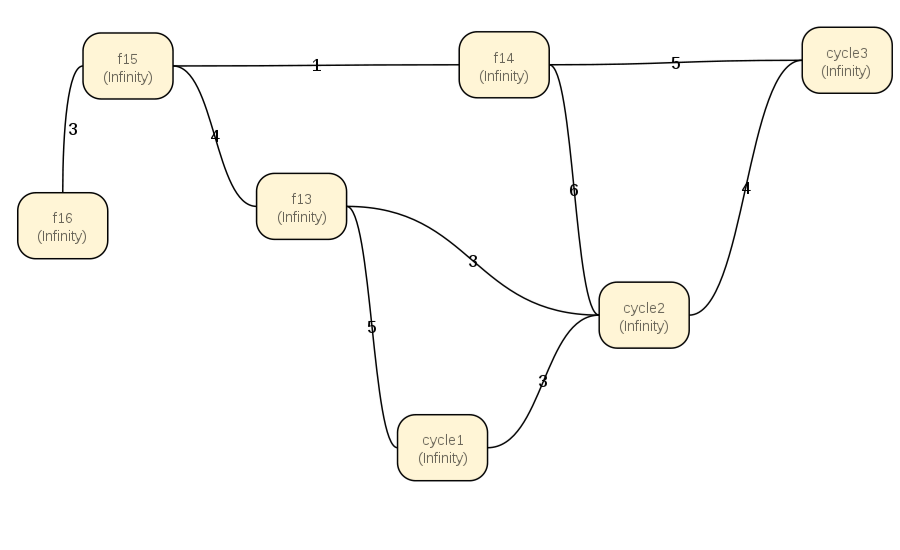
\includegraphics[width=0.8\textwidth,natwidth=800,natheight=800]{kai.png}
	\caption{Topology of Kai}
	\label{overflow}
\end{figure}
\begin{figure}
	\centering
	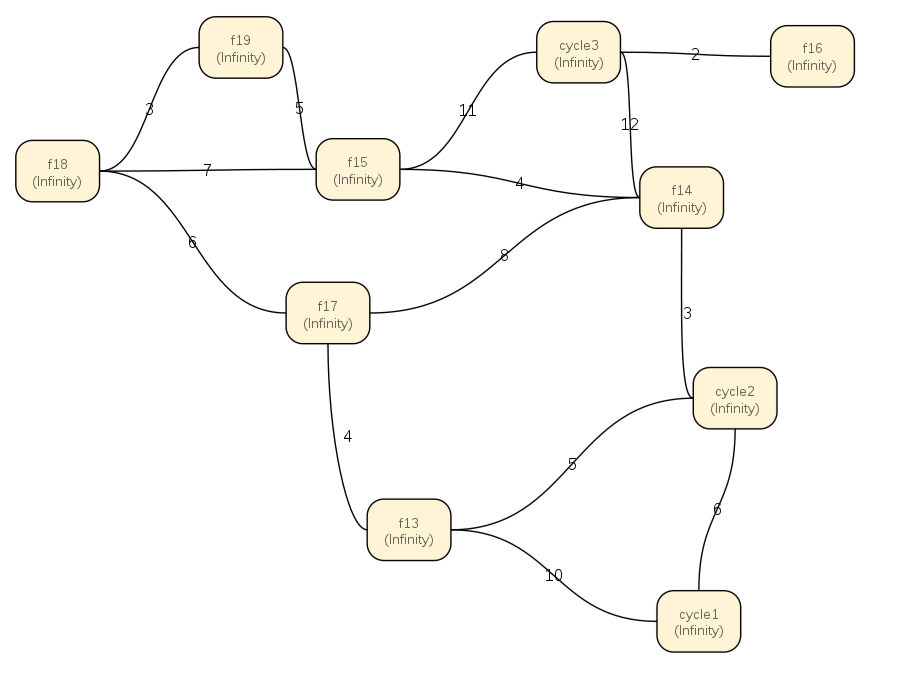
\includegraphics[width=0.8\textwidth,natwidth=900,natheight=900]{knex.png}
	\caption{Topology of Knex}
	\label{overflow}
\end{figure}
\begin{figure}
	\centering
	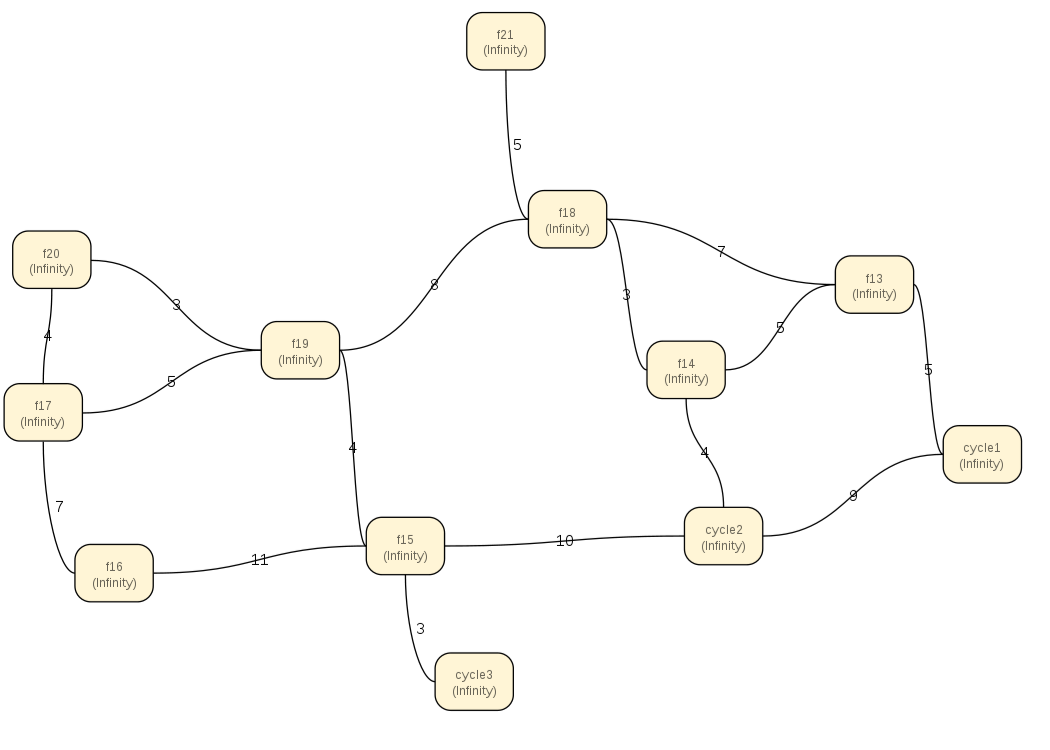
\includegraphics[width=0.8\textwidth,natwidth=1100,natheight=1100]{spaghetti.png}
	\caption{Topology of Spaghetti}
	\label{overflow}
\end{figure}

\end{document}
